\documentclass[11pt,a4paper]{article}

% ---------- Paquetes ----------
\usepackage[utf8]{inputenc}
\usepackage[T1]{fontenc}
\usepackage[spanish,es-tabla,es-nodecimaldot]{babel}
\usepackage[margin=2.5cm]{geometry}
\usepackage{booktabs}
\usepackage{array}
\usepackage{caption}
\usepackage{enumitem}
\usepackage{xcolor}
\usepackage{titlesec}
\usepackage{fancyhdr}
\usepackage{graphicx}
\usepackage{float}
\usepackage[colorlinks=true,linkcolor=black,citecolor=black,urlcolor=blue!50!black]{hyperref}
\newcommand{\dt}{.\allowbreak}
\newcommand{\us}{\_\allowbreak}
\newcommand{\var}[1]{\texttt{#1}}

\setlength{\parskip}{0.45em}
\setlength{\parindent}{0pt}
\captionsetup{font=small,labelfont=bf}
\renewcommand{\tablename}{Tabla}
\renewcommand{\arraystretch}{0.95}
\graphicspath{{../figures/}{../figures/eda/}}

\titleformat{\section}{\normalfont\Large\bfseries}{\thesection.}{0.6em}{}
\titleformat{\subsection}{\normalfont\large\bfseries}{\thesubsection}{0.6em}{}
\titlespacing*{\section}{0pt}{1.2em}{0.6em}

\pagestyle{fancy}
\fancyhf{}
\fancyhead[L]{\small Machine Learning II --- Proyecto Integrador}
\fancyhead[R]{\small Segunda Entrega}
\fancyfoot[C]{\small\thepage}
\renewcommand{\headrulewidth}{0.4pt}

% ---------- Datos del proyecto ----------
\newcommand{\tituloProyecto}{Predicción de deserción estudiantil en el Tecnológico de Monterrey mediante modelado avanzado de Machine Learning}
\newcommand{\nombreCurso}{Machine Learning II}
\newcommand{\nombreProfesor}{Wilmer Pineda}
\newcommand{\repo}{\url{https://github.com/miguel-camargo611/ML2-desercion-estudiantil}}

\begin{document}

% ================= PORTADA =================
\begin{titlepage}
\centering
\vspace*{1.5cm}
{\Large\bfseries Universidad Externado de Colombia\par}
\vspace{0.2cm}
{\large Departamento de Matemáticas\par}
\vspace{0.15cm}
{\large \nombreCurso\par}
\vspace{2.2cm}

{\large\scshape Proyecto Integrador --- Segunda Entrega\par}
\vspace{0.2cm}
{\normalsize Fase 2: datos, modelamiento y validación\par}
\vspace{0.4cm}
\rule{0.6\linewidth}{0.4pt}
\vspace{0.6cm}

{\Huge\bfseries \tituloProyecto \par}
\vspace{0.6cm}
\rule{0.6\linewidth}{0.4pt}

\vfill

\begin{minipage}{0.75\linewidth}
\centering
\textbf{Integrantes}\\[0.3cm]
Miguel Camargo \\
Camilo Hernández
\end{minipage}

\vspace{1.2cm}
\textbf{Profesor:} \nombreProfesor

\vspace{1.2cm}
{\large 2 de octubre de 2026 \par}
\vfill
\end{titlepage}

\pagenumbering{arabic}
\setcounter{page}{1}

% ================= INTRODUCCIÓN =================
Este informe corresponde a la segunda fase del proyecto: datos, modelamiento y validación. La pregunta es qué modelo predice mejor si un estudiante de pregrado dejará la universidad durante su primer año, usando lo que se sabe de él al terminar su primer semestre. Si la predicción es buena, la universidad puede ofrecer acompañamiento a tiempo a quienes más lo necesitan. El código y los pasos para repetir cada resultado se describen en el anexo.

% ================= SECCIÓN 1 =================
\section{Consolidación de los datos}

\textbf{Fuente.} Se usó el \textit{Student Dropout Dataset} del Tecnológico de Monterrey (Alvarado-Uribe et al., 2022), obtenido por solicitud formal al IFE Data Hub. Tiene 143.326 registros de estudiantes de bachillerato y pregrado que ingresaron entre agosto de 2014 (cohorte AD14) y agosto de 2020 (cohorte AD20). Son datos reales latinoamericanos, así que no fue necesario simular.

\textbf{Población de estudio y variable objetivo.} Villar y Andrade (2024) predicen la deserción con dos tipos de información: la que se conoce al ingresar y el desempeño en los primeros semestres. En este dataset, las notas del primer semestre (promedio, materias reprobadas y materias retiradas) solo existen para las cohortes AD19 y AD20 (Figura~\ref{fig:faltantes}). Por eso el estudio se concentra en los 24.251 estudiantes de pregrado de esas dos cohortes. La predicción se hace al terminar el primer semestre, y la variable objetivo vale 1 si el estudiante ya no está matriculado al cerrar su primer año. Se dejó por fuera a los 256 estudiantes que se retiraron a mitad del primer semestre: cuando se hace la predicción ya se fueron, y su promedio es bajo porque abandonaron, no al revés. El artículo distingue tres desenlaces (graduado, rezagado y desertor), pero este dataset no registra la graduación, así que el problema tiene dos clases: deserta o no. Solo deserta el 7,7\,\% de los estudiantes, frente al 32\,\% del artículo, y esa diferencia pesa en la elección de métricas (Sección~4).

\begin{figure}[H]
\centering
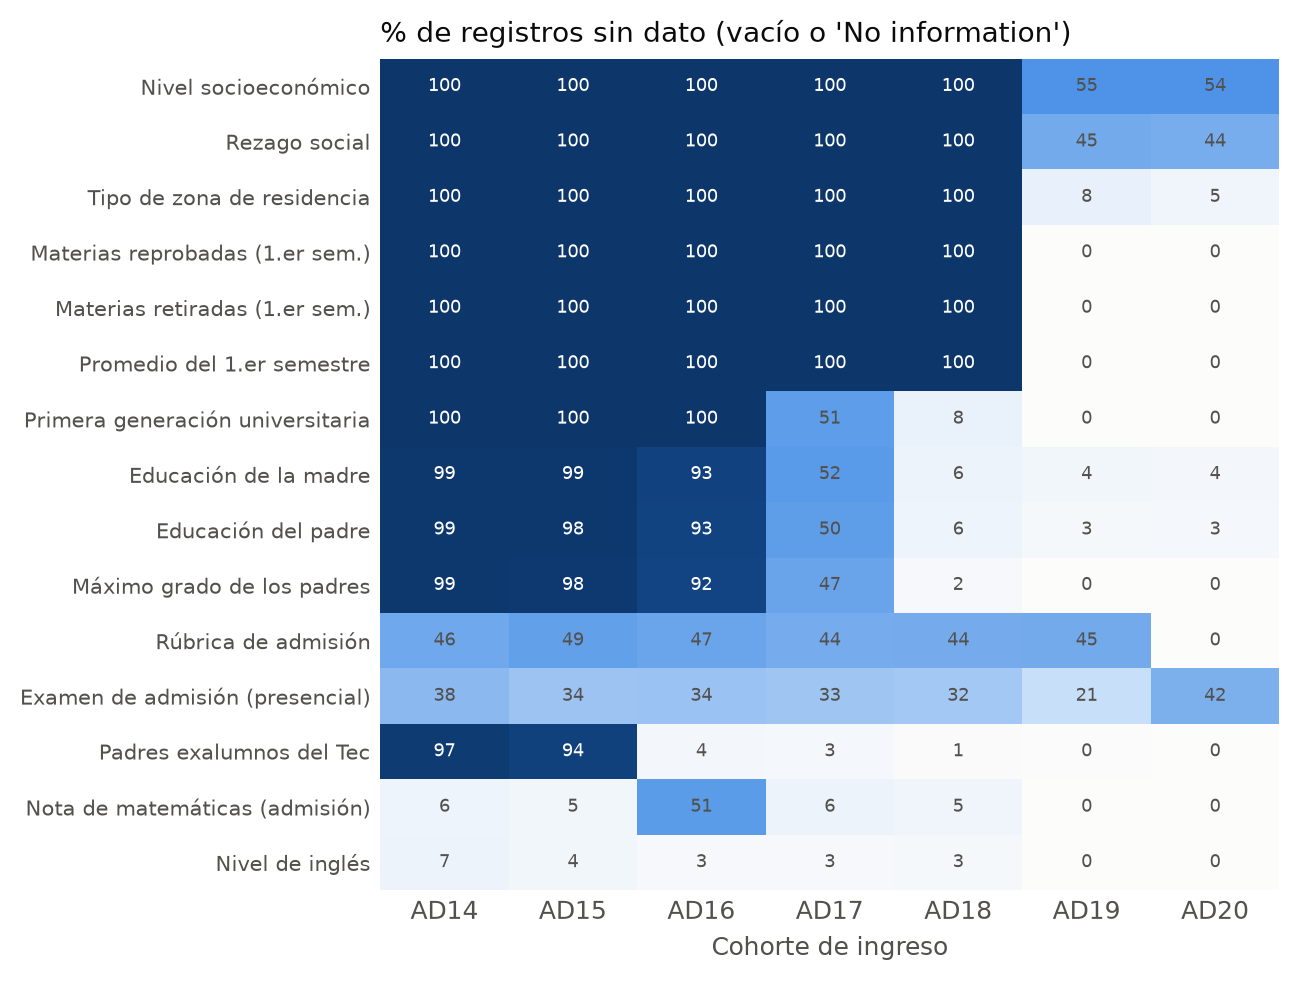
\includegraphics[width=0.72\linewidth]{eda02_faltantes_cohorte.png}
\caption{Porcentaje de registros sin dato por variable y cohorte (pregrado, conjunto de desarrollo). Los faltantes dependen de la cohorte: las notas del primer semestre solo existen en AD19 y AD20.}
\label{fig:faltantes}
\end{figure}

\textbf{Calidad de los datos.} El análisis exploratorio, disponible en el repositorio, encontró los problemas de la Tabla~\ref{tab:calidad}. El más relevante afecta a dos variables socioeconómicas, el nivel socioeconómico y el rezago social, que \textbf{no son utilizables}: falta el dato para cerca de la mitad de los estudiantes porque nunca se registró, la deserción es la misma con y sin dato, y cuando el dato existe casi no ayuda a distinguir a quienes desertan. Rellenar la mitad de una variable que no aporta solo agrega ruido, así que se excluyeron. La información familiar que sí está completa, la educación de los padres, se conservó.

\begin{table}[!t]
\centering
\footnotesize
\caption{Problemas de calidad encontrados en la población de estudio y decisión adoptada.}
\label{tab:calidad}
\begin{tabular}{>{\raggedright\arraybackslash}p{5.6cm}>{\raggedright\arraybackslash}p{2.4cm}>{\raggedright\arraybackslash}p{6.2cm}}
\toprule
Problema & Magnitud & Decisión \\
\midrule
Nivel socioeconómico y rezago social sin dato; la deserción es igual con y sin dato & 55\,\% y 44\,\% & Se excluyen: no son utilizables. \\
Examen de admisión con dos escalas: presencial (400--1600) y en línea (0--100) & 570 estudiantes en línea & Se separa en dos variables antes de modelar. \\
Puntajes de admisión faltantes; quienes no los tienen desertan más & 22--32\,\% & Se rellenan con la mediana y se agrega una variable que indica que faltaban. \\
\% total de apoyo económico, que es la suma de beca y crédito & $\rho=0{,}96$ & Se excluye por repetir información. \\
Actividades extracurriculares medidas \emph{durante} el año & 9 variables & Se excluyen: reflejan la permanencia en lugar de anticiparla. \\
Estudiantes que aparecen más de una vez & 6 casos & Cada estudiante queda en un solo lado de cada partición. \\
\bottomrule
\end{tabular}
\end{table}

\textbf{Variables construidas y selección.} Se creó una variable nueva, la \emph{brecha de promedios}: promedio del primer semestre menos promedio de bachillerato. Indica si el estudiante bajó o subió su rendimiento al llegar a la universidad. Quienes bajan más de siete puntos desertan un 18\,\%; quienes mantienen su nivel, un 5\,\%. Esta variable mejoró a LightGBM en las cinco particiones de validación. Se probó otra (materias reprobadas más retiradas), pero no aportó y se descartó. Después se midió cuánto empeora el modelo si se desordenan al azar los valores de cada variable (importancia por permutación), siempre con los datos de entrenamiento. Cinco variables no aportaban nada (tipo de zona, examen en línea, procedencia, colegio del Tec y primera generación) y se retiraron; en particiones nuevas, el modelo obtuvo el mismo resultado sin ellas (PR-AUC de 0,243). El modelo final usa 23 variables: 13 numéricas (promedios de bachillerato y del semestre, brecha, materias reprobadas y retiradas, examen, rúbrica y nota de matemáticas de admisión, nivel de inglés, porcentajes de beca y de crédito, edad y carga académica) y 10 categóricas (educación del padre y de la madre, máximo grado de los padres, padres exalumnos, costo del colegio, tipo de beca, escuela, programa, región y género). La Tabla~\ref{tab:escenarios} resume el tamaño de los datos.

\begin{table}[H]
\centering
\small
\caption{Tamaño de los conjuntos de datos. El conjunto de prueba se reserva para la entrega final.}
\label{tab:escenarios}
\begin{tabular}{lrrrr}
\toprule
Conjunto & Estudiantes & Desertores & Deserción & Variables \\
\midrule
Desarrollo (80\,\%) & 19.408 & 1.505 & 7,8\,\% & 23 \\
Prueba sellada (20\,\%) & 4.843 & 367 & 7,6\,\% & 23 \\
\bottomrule
\end{tabular}
\end{table}

% ================= SECCIÓN 2 =================
\section{Flujo reproducible sin fuga de datos}

Para que los resultados reflejen cómo funcionaría el modelo con estudiantes nuevos, se tomaron tres precauciones.

\textbf{1. Conjunto de prueba sellado.} Antes de cualquier análisis se apartó el 20\,\% de los estudiantes. Ese grupo no se ha mirado, ni siquiera en el análisis exploratorio, y solo se usará una vez, en la entrega final. Conserva la misma proporción de desertores y de cohortes, y cada estudiante queda en un solo lado.

\textbf{2. Preparación dentro de un \texttt{Pipeline}.} Todos los pasos van encadenados en este orden: (1) rellenar los datos faltantes con la mediana y marcar, con una variable adicional, que faltaban; (2) estandarizar las variables numéricas; (3) convertir las categóricas en columnas de ceros y unos (\textit{one-hot}), agrupando las categorías con menos de 30 estudiantes; (4) balancear las clases con SMOTE, si la validación lo elige, y (5) entrenar el modelo. La clave es que cada paso aprende solo de los datos de entrenamiento de cada partición (la mediana, la media, las categorías) y luego aplica lo aprendido, sin recalcular, a los datos de validación. Si la estandarización usara la media de todos los datos, el modelo ya tendría una pista de los estudiantes con que se evalúa. El orden también importa: se estandariza antes de SMOTE porque SMOTE crea estudiantes sintéticos a partir de los más parecidos, y para medir parecido las variables deben estar en la misma escala. Sin ese paso, el examen de admisión (hasta 1.600 puntos) pesaría mucho más que el porcentaje de beca (hasta 1). La regresión logística y la SVM también necesitan esa escala común; los árboles no, porque solo comparan valores dentro de una misma variable, y por eso CatBoost recibe los datos sin transformar. SMOTE actúa solo al entrenar, así que la validación conserva la proporción real de desertores. Pruebas automáticas del repositorio verifican que estos pasos aprenden únicamente de los datos de entrenamiento.

\textbf{3. Validación cruzada anidada.} Los datos de desarrollo se dividieron en cinco partes, sin repartir a un mismo estudiante entre dos partes y conservando la proporción de desertores. En cada una de cinco rondas, el modelo se entrena con cuatro partes y se evalúa con la quinta. Las decisiones (qué hiperparámetros usar y a partir de qué probabilidad emitir una alerta) se toman con nuevas divisiones internas de esas cuatro partes. Así, la parte con que se evalúa nunca influye en ninguna decisión. Los resultados se reportan como promedio y desviación estándar de las cinco rondas.

\textbf{Efecto de la fuga en el procedimiento del artículo.} Villar y Andrade aplican SMOTE a todos los datos antes de separar entrenamiento y validación. Para medir el efecto se entrenó el mismo modelo, LightGBM, de las dos maneras (Tabla~\ref{tab:fuga}). Con el procedimiento del artículo, el F1 de la clase deserción es de 0,95; con el nuestro, de 0,12. La razón es sencilla: SMOTE crea desertores sintéticos mezclando desertores reales. Si se crean antes de separar, los desertores de validación son mezclas de estudiantes que el modelo ya vio, y acertar es fácil. Esto sugiere que parte del alto desempeño del artículo (F1 de 0,83 a 0,88) viene del procedimiento y no del modelo.

\begin{table}[H]
\centering
\small
\caption{Mismo modelo evaluado con los dos procedimientos (cinco rondas). El PR-AUC se explica en la Sección~4.}
\label{tab:fuga}
\begin{tabular}{lcc}
\toprule
Protocolo & F1 deserción (umbral 0,5) & PR-AUC \\
\midrule
SMOTE antes de separar (artículo) & 0{,}95 & 0{,}98 \\
SMOTE solo en entrenamiento (este trabajo) & 0{,}12 & 0{,}24 \\
\bottomrule
\end{tabular}

\end{table}

% ================= SECCIÓN 3 =================
\section{Reproducción y adaptación del método}

El método del artículo compara árboles y ensambles clásicos con cuatro algoritmos de \textit{boosting}, equilibra las clases con SMOTE (Chawla et al., 2002), ajusta los hiperparámetros e interpreta el mejor modelo con SHAP (Lundberg y Lee, 2017). La Tabla~\ref{tab:adaptacion} resume qué se conservó, qué se cambió y por qué.

\begin{table}[H]
\centering
\footnotesize
\caption{Reproducción y adaptación del método de Villar y Andrade (2024).}
\label{tab:adaptacion}
\begin{tabular}{>{\raggedright\arraybackslash}p{2.5cm}>{\raggedright\arraybackslash}p{4.6cm}>{\raggedright\arraybackslash}p{7.1cm}}
\toprule
Elemento & Artículo & Este trabajo \\
\midrule
Información & Ingreso + desempeño de los primeros semestres & Ingreso + desempeño del primer semestre (cohortes AD19--AD20) \\
Variable objetivo & Tres clases: graduado, rezagado y desertor & Dos clases: deserta o no en el primer año (el dataset no registra la graduación) \\
Modelos & Árbol, Random Forest, SVM, Gradient Boosting, XGBoost, LightGBM, CatBoost & Los mismos, más la regresión logística como referencia \\
Balanceo de clases & SMOTE sobre todos los datos & SMOTE solo sobre el entrenamiento, y como una opción más: la validación decide si se usa \\
Hiperparámetros & Optuna & \texttt{GridSearchCV}, herramienta del curso, dentro de la validación anidada \\
Métrica principal & F1 ponderado & PR-AUC, más \textit{recall} y precisión de la clase deserción \\
Comparación & Prueba t pareada & Prueba t corregida de Nadeau y Bengio (2003) \\
Interpretación & SHAP & SHAP, repetido en cada ronda para comprobar su estabilidad \\
\bottomrule
\end{tabular}
\end{table}

\textbf{Modelos comparados.} Se compararon nueve modelos. Dos son líneas base: uno que asigna a todos la misma probabilidad de desertar y un árbol de decisión sin poda. La regresión logística sirve de referencia, porque es el modelo de Machine Learning I. Los otros seis son los del artículo: Random Forest, SVM con kernel RBF, Gradient Boosting, XGBoost, LightGBM y CatBoost. CatBoost trabaja directamente con las variables categóricas, sin convertirlas en ceros y unos; como SMOTE no funciona con ese tipo de variables, en su caso el desbalance se trata dando más peso a los desertores. Para que la SVM fuera viable con casi 20.000 estudiantes, se usó una aproximación de su kernel (Nystroem).

\textbf{Ajuste de hiperparámetros.} Cada modelo tiene una rejilla de hiperparámetros que controlan qué tan complejo puede ser (Tabla~\ref{tab:hiper}). En cada ronda, \texttt{GridSearchCV} probó todas las combinaciones, de 4 a 24 según el modelo, y eligió la de mayor PR-AUC. Usar o no SMOTE se trató como una opción más de la rejilla, y el resultado es claro: la validación \textbf{no eligió SMOTE en ninguna de las 30 decisiones} (seis modelos por cinco rondas), y CatBoost tampoco eligió dar más peso a los desertores. Crear desertores sintéticos no ayuda a ordenar a los estudiantes por riesgo; el desbalance se maneja mejor al fijar el umbral de alerta (Sección~4). Las configuraciones elegidas son simples: árboles poco profundos y regularización fuerte. La Figura~\ref{fig:curvas} explica por qué. Cuando LightGBM puede usar árboles más grandes, su resultado en entrenamiento sube de 0,24 a 0,91, pero en validación solo mejora hasta las 8 hojas por árbol (0,250) y luego empeora: el modelo empieza a memorizar casos en lugar de aprender patrones. En la SVM, los valores elegidos quedaron en el borde de la rejilla, pero la curva muestra que ampliar $C$ a 1 ya no mejora (0,232 frente a 0,235). Por su alto costo (Sección~4), la rejilla de CatBoost se limitó a la profundidad y al peso de los desertores.

\begin{figure}[H]
\centering
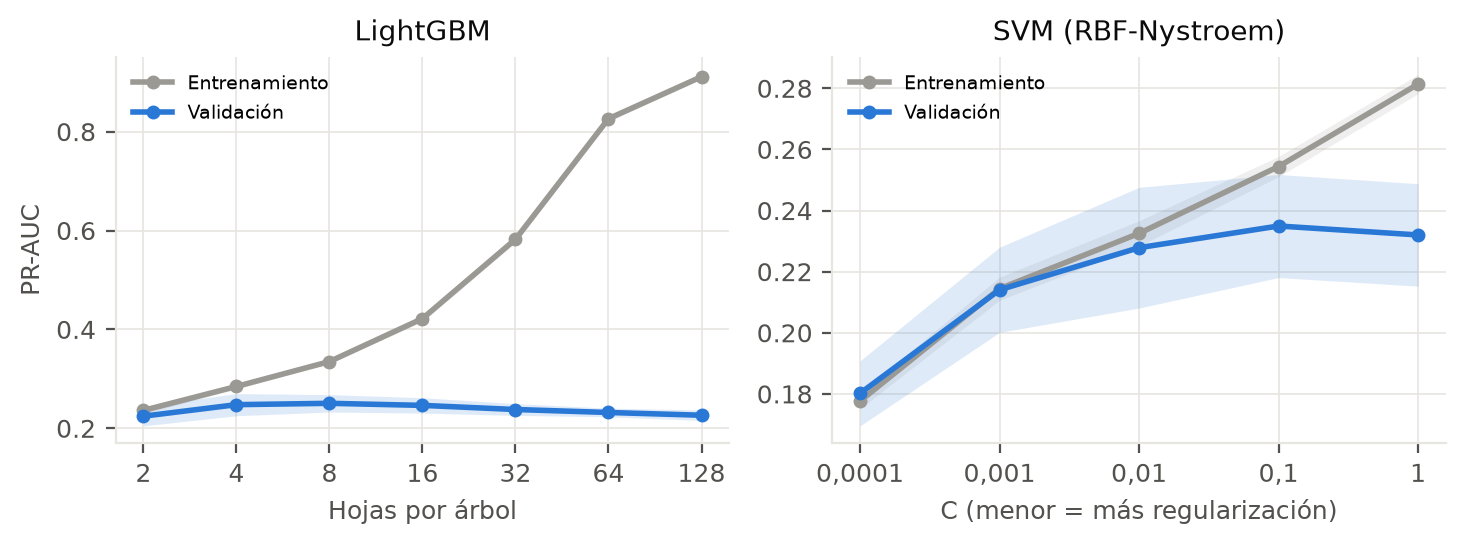
\includegraphics[width=0.86\linewidth]{fig06_curva_validacion.png}
\caption{Curvas de validación alrededor de la configuración elegida (media $\pm$ desviación estándar de cinco rondas). Cuando la distancia entre entrenamiento y validación crece, el modelo está memorizando.}
\label{fig:curvas}
\end{figure}

\begin{table}[H]
\centering
\footnotesize
\caption{Hiperparámetros explorados y combinación elegida con más frecuencia (entre paréntesis, en cuántas de las cinco rondas se eligió).}
\label{tab:hiper}
\begin{tabular}{>{\raggedright\arraybackslash}p{2.4cm}>{\raggedright\arraybackslash}p{8.2cm}>{\raggedright\arraybackslash}p{3.6cm}}
\toprule
Modelo & Valores explorados & Elegido (rondas) \\
\midrule
Regresión logística & $C$: 0{,}0001, 0{,}0003, 0{,}001, 0{,}003, 0{,}01, 0{,}03, 0{,}1; balanceo: ninguno, SMOTE & 0{,}03, ninguno (2/5) \\
Random Forest & mín. registros por hoja: 5, 15, 40, 100; variables por división: $\sqrt{p}$, 0{,}4; balanceo: ninguno, SMOTE & 15, 0{,}4, ninguno (2/5) \\
SVM (kernel RBF) & $\gamma$: 0{,}001, 0{,}003, 0{,}01; $C$: 0{,}001, 0{,}01, 0{,}1; balanceo: ninguno, SMOTE & 0{,}01, 0{,}1, ninguno (5/5) \\
Gradient Boosting & tasa de aprendizaje: 0{,}02, 0{,}05; máx. hojas: 4, 8, 16; regularización L2: 0, 1; balanceo: ninguno, SMOTE & 0{,}05, 4, 1, ninguno (4/5) \\
XGBoost & profundidad máx.: 2, 3, 4; tasa de aprendizaje: 0{,}02, 0{,}05; peso mín. por hoja: 1, 10; balanceo: ninguno, SMOTE & 2, 0{,}05, 1, ninguno (4/5) \\
LightGBM & hojas: 4, 8, 16; tasa de aprendizaje: 0{,}02, 0{,}05; mín. registros por hoja: 20, 100; balanceo: ninguno, SMOTE & 4, 0{,}02, 100, ninguno (2/5) \\
CatBoost & profundidad: 4, 6; pesos de clase: ninguno, balanceados & 4, ninguno (4/5) \\
\bottomrule
\end{tabular}

\end{table}

\textbf{Otros elementos del artículo.} (i) \emph{SMOTE frente a ADASYN.} Como en el artículo, con un árbol de decisión SMOTE fue algo mejor que ADASYN (F1 de la clase deserción de 0,154 frente a 0,148), pero el árbol sin balanceo superó a ambos (0,162). (ii) \emph{Isolation Forest.} El artículo lo usa para ver si los desertores son estudiantes atípicos. Aquí tampoco lo son: el método casi no los distingue (ROC-AUC de 0,55, cuando 0,5 equivale al azar). (iii) \emph{Regresión logística.} El artículo la descartó porque varias variables repetían información (multicolinealidad). Aquí ocurrió lo mismo, y la causa era concreta: el porcentaje total de apoyo es la suma exacta de beca y crédito. Al quitar ese total, el problema desaparece (el VIF de la beca baja de 10\textsuperscript{7} a 1,3) y el modelo se pudo conservar. La brecha de promedios también es la resta de dos variables del modelo, pero se dejó a propósito: a los árboles les sirve, porque analizan una variable a la vez y no pueden calcular esa resta por sí solos; a la regresión logística no le aporta, pero su regularización evita que la repetición la desestabilice.

\textbf{Por qué no se usaron modelos de densidad ni de clustering.} La Primera entrega los dejó para más adelante, según el calendario del curso, pero al final no se incluyeron, por tres razones. Primera, la guía del proyecto pide comparar modelos según el artículo, y el artículo solo usa un método de este tipo, Isolation Forest, que sí se replicó. Segunda, ese resultado muestra que los desertores no forman un grupo aparte ni atípico en los datos, que es justo lo que un enfoque de densidad necesitaría para funcionar. Tercera, el problema es supervisado: el clustering agrupa estudiantes sin mirar si desertaron, y nada garantiza que esos grupos separen a quienes se van. Además, modelos como las mezclas gaussianas suponen variables continuas con forma de campana, y aquí 10 de las 23 variables son categóricas.

% ================= SECCIÓN 4 =================
\section{Validación, métricas e interpretación preliminar}

\textbf{Métricas.} Con solo 7,8\,\% de desertores, el F1 ponderado que usa el artículo engaña: un modelo que no alerta a nadie obtiene 0,89 sin encontrar a un solo desertor. Por eso los modelos se compararon con el PR-AUC, que mide qué tan bien ordenan a los estudiantes de mayor a menor riesgo (el azar obtiene 0,078 y un modelo perfecto, 1). También se reportan el \textit{recall}, la parte de los desertores que se detecta, y la precisión, la parte de las alertas que acierta. La alerta se emite cuando la probabilidad estimada supera un umbral, que se eligió con los datos de entrenamiento para maximizar F2, una medida que da al \textit{recall} el doble de peso que a la precisión. Así se traduce la prioridad fijada en la Primera entrega: dejar pasar a un desertor cuesta más que acompañar a un estudiante que no lo necesitaba.

\textbf{Resultados.} La Tabla~\ref{tab:resultados} y la Figura~\ref{fig:comparacion} resumen el desempeño. Todos los modelos avanzados superan con claridad a las líneas base. El árbol sin poda queda casi al nivel del azar (0,091 frente a 0,078) porque memoriza los datos de entrenamiento. Las líneas base aparecen con \textit{recall} de 1,00 porque dan a todos la misma probabilidad (o casi), así que el umbral termina alertando a todos; por eso se comparan por PR-AUC. Entre los modelos avanzados, los de \textit{boosting} encabezan y están prácticamente empatados: CatBoost (0,248), XGBoost (0,248), LightGBM (0,247) y Gradient Boosting (0,245). Les siguen la SVM (0,235), Random Forest (0,230) y la regresión logística (0,224). Que todos ronden una ROC-AUC de 0,72 confirma lo que mostró el análisis exploratorio: los datos contienen una señal real, pero débil y repartida entre muchas variables.

\begin{table}[H]
\centering
\footnotesize
\caption{Resultados de la validación cruzada anidada: PR-AUC y ROC-AUC (promedio $\pm$ desviación estándar de las cinco rondas); \textit{recall}, precisión y proporción de estudiantes alertados con el umbral elegido. En negrita, el mejor PR-AUC.}
\label{tab:resultados}
\begin{tabular}{lrrrrr}
\toprule
Modelo & PR-AUC & ROC-AUC & Recall & Precisión & Alertas \\
\midrule
Mayoría & 0{,}078\,\scriptsize$\pm$0{,}000 & 0{,}500\,\scriptsize$\pm$0{,}000 & 1{,}00 & 0{,}08 & 1{,}00 \\
Árbol sin poda & 0{,}091\,\scriptsize$\pm$0{,}005 & 0{,}546\,\scriptsize$\pm$0{,}011 & 1{,}00 & 0{,}08 & 1{,}00 \\
\midrule
Regresión logística & 0{,}224\,\scriptsize$\pm$0{,}019 & 0{,}715\,\scriptsize$\pm$0{,}010 & 0{,}64 & 0{,}14 & 0{,}36 \\
Random Forest & 0{,}230\,\scriptsize$\pm$0{,}018 & 0{,}697\,\scriptsize$\pm$0{,}012 & 0{,}58 & 0{,}14 & 0{,}33 \\
SVM (kernel RBF) & 0{,}235\,\scriptsize$\pm$0{,}017 & 0{,}716\,\scriptsize$\pm$0{,}007 & 0{,}63 & 0{,}14 & 0{,}36 \\
Gradient Boosting & 0{,}245\,\scriptsize$\pm$0{,}022 & 0{,}716\,\scriptsize$\pm$0{,}007 & 0{,}68 & 0{,}13 & 0{,}40 \\
XGBoost & 0{,}248\,\scriptsize$\pm$0{,}021 & 0{,}717\,\scriptsize$\pm$0{,}009 & 0{,}60 & 0{,}14 & 0{,}33 \\
LightGBM & 0{,}247\,\scriptsize$\pm$0{,}023 & 0{,}716\,\scriptsize$\pm$0{,}005 & 0{,}67 & 0{,}13 & 0{,}40 \\
CatBoost & \textbf{0{,}248\,\scriptsize$\pm$0{,}023} & 0{,}711\,\scriptsize$\pm$0{,}009 & 0{,}66 & 0{,}13 & 0{,}39 \\
\bottomrule
\end{tabular}

\end{table}

\begin{figure}[H]
\centering
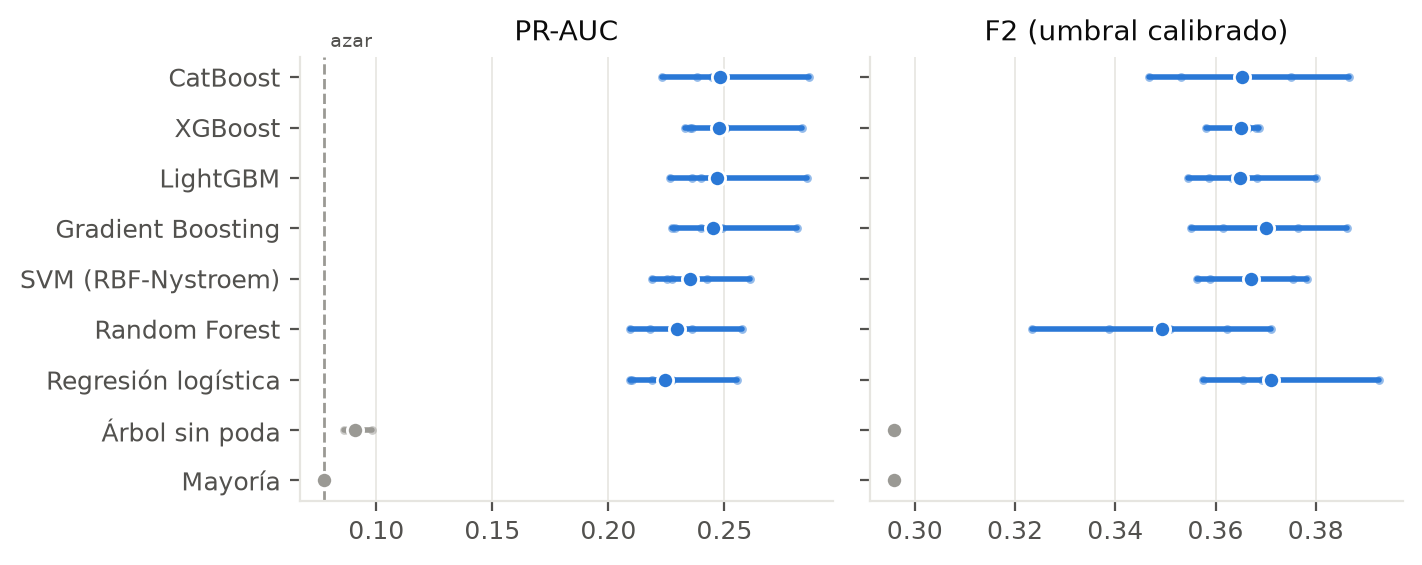
\includegraphics[width=0.86\linewidth]{fig03_comparacion_modelos.png}
\caption{PR-AUC y F2 de cada modelo en las cinco rondas (puntos pequeños) y su promedio (punto grande). La línea punteada es el PR-AUC de un modelo al azar.}
\label{fig:comparacion}
\end{figure}

\textbf{\textquestiondown{}Son reales las diferencias?} Las cinco rondas comparten buena parte de sus datos de entrenamiento, así que sus resultados no son independientes. La prueba t corregida de Nadeau y Bengio (2003) tiene en cuenta ese solapamiento; la prueba t pareada del artículo, no. Con la prueba corregida, CatBoost no se distingue de XGBoost, LightGBM ni Gradient Boosting ($p \geq 0{,}44$), ni con claridad de la SVM ($p=0{,}09$) o de Random Forest ($p=0{,}13$); sí supera a la regresión logística ($p=0{,}026$) y a las líneas base ($p<0{,}001$). Con la prueba sin corregir, las diferencias con la SVM y Random Forest habrían parecido reales ($p=0{,}030$ y $0{,}047$). En resumen, el \textit{boosting} mejora a un buen modelo lineal, pero poco.

\textbf{Costo computacional.} Si varios modelos empatan, conviene preferir el más barato (Tabla~\ref{tab:costo}). CatBoost, primero por un margen mínimo, es el más lento: tarda 16 segundos en entrenarse y su búsqueda de hiperparámetros tomó 30 minutos con solo cuatro combinaciones. LightGBM logra el mismo resultado entrenándose en medio segundo y probando 24 combinaciones en 5,5 minutos. Random Forest ocupa 27 MB, frente a menos de 0,4 MB de los modelos de \textit{boosting}. Predecir es rápido con todos: menos de 16 milisegundos por cada mil estudiantes.

\begin{table}[H]
\centering
\footnotesize
\caption{Costo computacional (procesador de 12 hilos). Búsqueda: validación cruzada anidada completa. Ajuste y predicción: modelo final con los hiperparámetros elegidos, sobre los 19.408 estudiantes de desarrollo (mediana de tres repeticiones).}
\label{tab:costo}
\resizebox{\linewidth}{!}{\begin{tabular}{lrrrrrr}
\toprule
Modelo & PR-AUC & Combinaciones & Búsqueda (min) & Ajuste (s) & Predicción (ms/1.000) & Tamaño (MB) \\
\midrule
Mayoría & 0{,}078 & 1 & 0{,}4 & 0{,}20 & 2{,}9 & 0{,}01 \\
Árbol sin poda & 0{,}091 & 1 & 0{,}3 & 0{,}44 & 2{,}9 & 0{,}32 \\
Regresión logística & 0{,}224 & 14 & 1{,}5 & 0{,}30 & 3{,}4 & 0{,}01 \\
Random Forest & 0{,}230 & 16 & 24{,}9 & 4{,}57 & 14{,}9 & 26{,}90 \\
SVM (kernel RBF) & 0{,}235 & 18 & 3{,}9 & 2{,}35 & 15{,}7 & 2{,}31 \\
Gradient Boosting & 0{,}245 & 24 & 6{,}0 & 1{,}23 & 9{,}2 & 0{,}23 \\
XGBoost & 0{,}248 & 24 & 11{,}8 & 1{,}02 & 5{,}6 & 0{,}37 \\
LightGBM & 0{,}247 & 24 & 5{,}5 & 0{,}55 & 7{,}1 & 0{,}25 \\
CatBoost & 0{,}248 & 4 & 29{,}7 & 15{,}96 & 5{,}4 & 0{,}21 \\
\bottomrule
\end{tabular}
}
\end{table}

\textbf{Qué significa en la práctica.} Con el umbral elegido, CatBoost detecta al 66\,\% de los desertores, pero alerta al 39\,\% de los estudiantes, y solo 13 de cada 100 alertas son desertores reales. Es más útil pensarlo así: si la universidad solo puede acompañar al 20\,\% de estudiantes con mayor riesgo, el modelo le permite llegar al 46\,\% de quienes van a desertar, 2,3 veces más que eligiendo al azar. Si acompaña al 10\,\%, llega al 32\,\%, y una de cada cuatro alertas es correcta.

\textbf{Variables más influyentes.} Para saber en qué se basa el modelo se usó SHAP, que reparte cada predicción entre las variables. Se calculó en las cinco rondas para comprobar que las conclusiones no cambian con los datos. El promedio del primer semestre fue la variable más influyente en cuatro rondas, y el porcentaje de beca en la restante; después vienen el promedio de bachillerato, la rúbrica de admisión, el programa y la nota de matemáticas. La Figura~\ref{fig:shap} muestra en qué dirección actúa cada una: un promedio del semestre bajo sube mucho el riesgo, mientras que uno alto lo baja poco; las becas altas y un buen desempeño previo lo reducen; tener más edad y bajar el rendimiento respecto al bachillerato lo aumentan. Es el mismo hallazgo central del artículo: el desempeño académico temprano es el mejor predictor de la deserción. Son asociaciones útiles para predecir, no causas.

\begin{figure}[H]
\centering
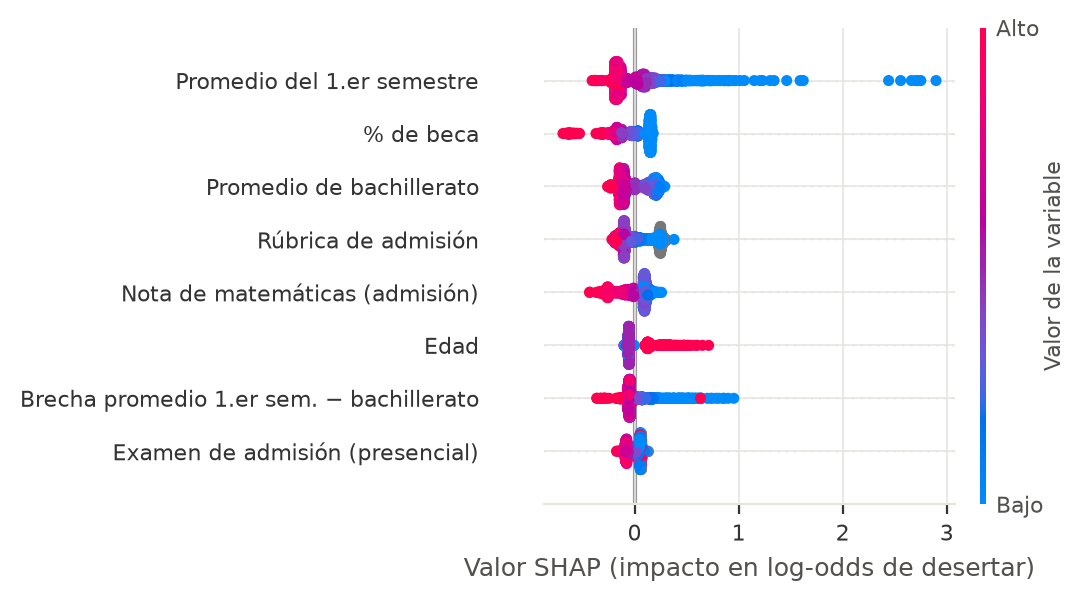
\includegraphics[width=0.8\linewidth]{fig08_shap_beeswarm.png}
\caption{Valores SHAP de CatBoost para las variables numéricas más influyentes (2.000 estudiantes de validación de la última ronda). Cada punto es un estudiante; los valores positivos aumentan el riesgo estimado de desertar.}
\label{fig:shap}
\end{figure}

\textbf{Errores e implicaciones.} El modelo casi no detecta a los desertores con beca por talento académico (6 de cada 100): como grupo tienen bajo riesgo, y lo que los lleva a irse no está en los datos. En cambio, alerta al 59\,\% de los estudiantes sin beca que no desertan. Por eso el modelo sirve para decidir a quién acompañar primero, no para etiquetar a los estudiantes, ya que varias de sus señales reflejan la situación económica.

\textbf{Pasos para la entrega final.} Evaluar una sola vez el modelo elegido, con su umbral ya fijado, en el conjunto de prueba; profundizar la interpretación, y desplegarlo en una aplicación de Streamlit que explique cada predicción.

\textbf{Código y uso de IA.} El análisis se hizo en Python con scikit-learn (Pedregosa et al., 2011), imbalanced-learn (Lemaître et al., 2017), XGBoost (Chen y Guestrin, 2016), LightGBM (Ke et al., 2017), CatBoost (Prokhorenkova et al., 2018) y SHAP. Se utilizó un asistente de inteligencia artificial (Claude, de Anthropic) como apoyo en la escritura del código y la revisión del texto; los autores verificaron los resultados y pueden sustentar cada decisión técnica.

% ================= BIBLIOGRAFÍA =================
\begin{thebibliography}{10}
\footnotesize
\setlength{\itemsep}{1pt}

\bibitem{alvarado2022}
Alvarado-Uribe, J., Mejía-Almada, P., Masetto Herrera, A. L., Molontay, R., Hilliger, I., Hegde, V., Montemayor Gallegos, J. E., Ramírez Díaz, R. A., \& Ceballos, H. G. (2022). Student Dataset from Tecnologico de Monterrey in Mexico to Predict Dropout in Higher Education. \textit{Data}, 7(9), 119. \url{https://doi.org/10.3390/data7090119}

\bibitem{chawla2002}
Chawla, N. V., Bowyer, K. W., Hall, L. O., \& Kegelmeyer, W. P. (2002). SMOTE: synthetic minority over-sampling technique. \textit{Journal of Artificial Intelligence Research}, 16, 321--357.

\bibitem{chen2016}
Chen, T. \& Guestrin, C. (2016). XGBoost: A scalable tree boosting system. En \textit{Proceedings of the 22nd ACM SIGKDD International Conference on Knowledge Discovery and Data Mining} (pp. 785--794).

\bibitem{ke2017}
Ke, G., Meng, Q., Finley, T., Wang, T., Chen, W., Ma, W., Ye, Q., \& Liu, T.-Y. (2017). LightGBM: A highly efficient gradient boosting decision tree. \textit{Advances in Neural Information Processing Systems}, 30.

\bibitem{lemaitre2017}
Lemaître, G., Nogueira, F., \& Aridas, C. K. (2017). Imbalanced-learn: A Python toolbox to tackle the curse of imbalanced datasets in machine learning. \textit{Journal of Machine Learning Research}, 18(17), 1--5.

\bibitem{lundberg2017}
Lundberg, S. M. \& Lee, S.-I. (2017). A unified approach to interpreting model predictions. \textit{Advances in Neural Information Processing Systems}, 30.

\bibitem{nadeau2003}
Nadeau, C. \& Bengio, Y. (2003). Inference for the generalization error. \textit{Machine Learning}, 52(3), 239--281.

\bibitem{pedregosa2011}
Pedregosa, F., Varoquaux, G., Gramfort, A., Michel, V., Thirion, B., Grisel, O., et al. (2011). Scikit-learn: Machine learning in Python. \textit{Journal of Machine Learning Research}, 12, 2825--2830.

\bibitem{prokhorenkova2018}
Prokhorenkova, L., Gusev, G., Vorobev, A., Dorogush, A. V., \& Gulin, A. (2018). CatBoost: unbiased boosting with categorical features. \textit{Advances in Neural Information Processing Systems}, 31.

\bibitem{villar2024}
Villar, A. \& Robledo Velini de Andrade, C. (2024). Supervised machine learning algorithms for predicting student dropout and academic success: a comparative study. \textit{Discover Artificial Intelligence}, 4:2. \url{https://doi.org/10.1007/s44163-023-00079-z}

\end{thebibliography}

% ================= ANEXO =================
\section*{Anexo: código y reproducibilidad}

El código está en \repo. Para repetir todos los resultados de este informe:
\begin{enumerate}[leftmargin=1.5em,itemsep=1pt,topsep=2pt]
\item Instalar el entorno con \texttt{pip install -e .} (las versiones de las librerías están fijadas).
\item Solicitar el dataset al TEC DataHub y copiar el archivo de Excel recibido en la carpeta \texttt{data/raw/}.
\item Ejecutar \texttt{desercion all}.
\end{enumerate}
Todo el flujo usa la semilla 42, de modo que se obtienen las mismas cifras. El análisis exploratorio completo está en \texttt{notebooks/01\us exploracion\us datos.ipynb}, y las pruebas automáticas (\texttt{pytest}) verifican, con datos sintéticos, que la preparación de los datos no filtra información de validación.

\end{document}
